\chapter{Cellular automata}

%Nejaka citacia od Feynmana o CA, neznali CA budu prekvapeni: \cite{Andel07}

Years before DNA and replication mechanism was discovered in living cells,
John von Neumann was investigating self-replicating systems in theory, 
and layed basis for the "New kind of science" \cite{wolfram}. 

%It seems that there is some truth in this statement. One search of "cellular automata" on Arxiv outputs thousands of articles on application and theory of cellular automata only from recent years.

%However, for many colleague-scientist remain cellular automata "velkou neznamou".
%What the essence of cellular automata can be easily explained on the following famous example.

\section{Game of Life}

John Conway, by significant simplification of von Neumann ideas, conceived the Game of Life in 1970, that renewed general interest in cellular automata.

Depending on the initial conditions, evolution of this automaton can be chaotic, periodic or it can lead to the stable configurations.

The reason for this complexity and diversity hides in the fundamental property that Game of Life posses - it is the Turing-complete, so in principle any program or computation that can be run on a computer can be simulated in Game of Life.   

For the purposes of this thesis, we have written a simple program implementing this game, as it easily expresses basic principles of cellular automata.

Let us have a rectangular grid, with black and white squares. 
White squares represent dead cells, black cells represent living cells.
On Fig.\ref{gol1} we see such grid, that we chose for initial state of 'Life'.


\begin{figure}[htbp]
 \centering
 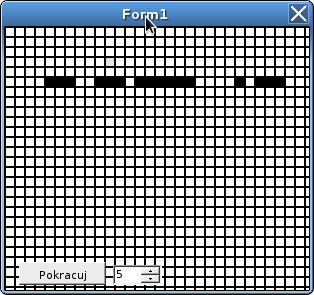
\includegraphics[width=0.7\textwidth]{./img/gol1}
 \label{gol1}
 \caption{The initial state of 'Life' (at t=0)}
\end{figure}

%The evolution of grid for our particular initial state is shown in figure blabla.\\  

Now we press 'Pokracuj' button and let the the Life evolve.

\begin{figure}
 \centering
 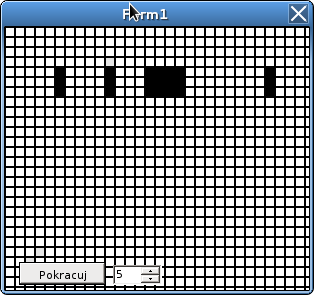
\includegraphics[width=0.7\textwidth]{./img/gol2}
 \label{gol2}
 \caption{t=1}
\end{figure}

\begin{figure}
 \centering
 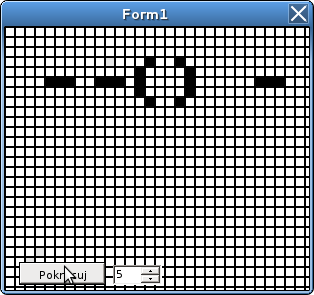
\includegraphics[width=0.7\textwidth]{./img/gol3}
 \label{gol2}
 \caption{t=2}
\end{figure}

In the discrete time steps, the grid is changing.
We see some that cells are dying, but some cells are getting alive. 
What is the rule that kills the cell or leave it be? 
It depends on the state of the cell itself and state of it eight neighbouring cells.
\begin{enumerate}
\item If the cell is alive, and 2 or 3 neighbouring cells are alive, cell will stay alive in the next step, otherwise it will die.
\item If the cell is dead, and EXACTLY 3 neighbouring cells are alive, the cell will get alive in the next step.
\item All other configurations do not change state of the cell.

\end{enumerate}


Let us proceed from this simple example to more general approach.
In the next chapter, we will generalize main features of 'Life' and formally define the cellular automaton.
%In the next chapter, we will generalize main feature of 'Life'
%Let us generalize this example into formal definition of cellular automaton.

\section{Formal definition}
\textbf{Position of cells:}

Instead of 2D rectangular grid from 'Life',
cells might be arranged in arbitrary N dimensional
regular grid, not necessary rectangular. 
(Regularity follows from definition of Kubrid. In general, cells might be positioned really wildly,
e.g. on Penrose lattice, or arbritrary as proposed by Richard P. Feynman).
\bigskip

\textbf{Set of cell states Q:}

In 'Life' cells can be dead or alive (set of states has cardinality 2). 
In general CA, set of states can be any finite set Q of cardinality K.
%cell can be in one of K states from the finiteset of states. 
%We will mark set of states Q, and use this in definition of upgrade rule later.
\bigskip

\textbf{Neighborhood:}

In 'Life', state of the cell in the next step was determined
by 8 neighbouring cells. We call these cells neighborhood of range r = 1 (in the distance of 1 cell).
For general CA, we might consider neighborhood
with arbitrary range.
(Neighborhood with r = 2 in 'Life' would involve 9+16=25 cells).

\bigskip

\textbf{Update rule:}

Update rule is an arbitrary bounded mapping U from Neighborhood to the set of states Q.
Since the state of the Cell is determined only by the state of its Neighborhood, update rules in CA are local.

\section{The most basic cellular automaton} 

In middle 1980s, on the prestigious Princeton institute,
Stephen Wolfram and his assistants were performing unusual computer experiments \cite{levy} and analyzing the patterns by 1D cellular automata (to a despair of their senior colleagues)\cite{levy}.

The most basic CA is 1D CA with range r=1 and its cells can be in one of two states (alive or dead).

1D CA means, that cells are arranged in the row, see Fig.~\ref{1d}

\begin{figure}[htbp]
 \centering 
 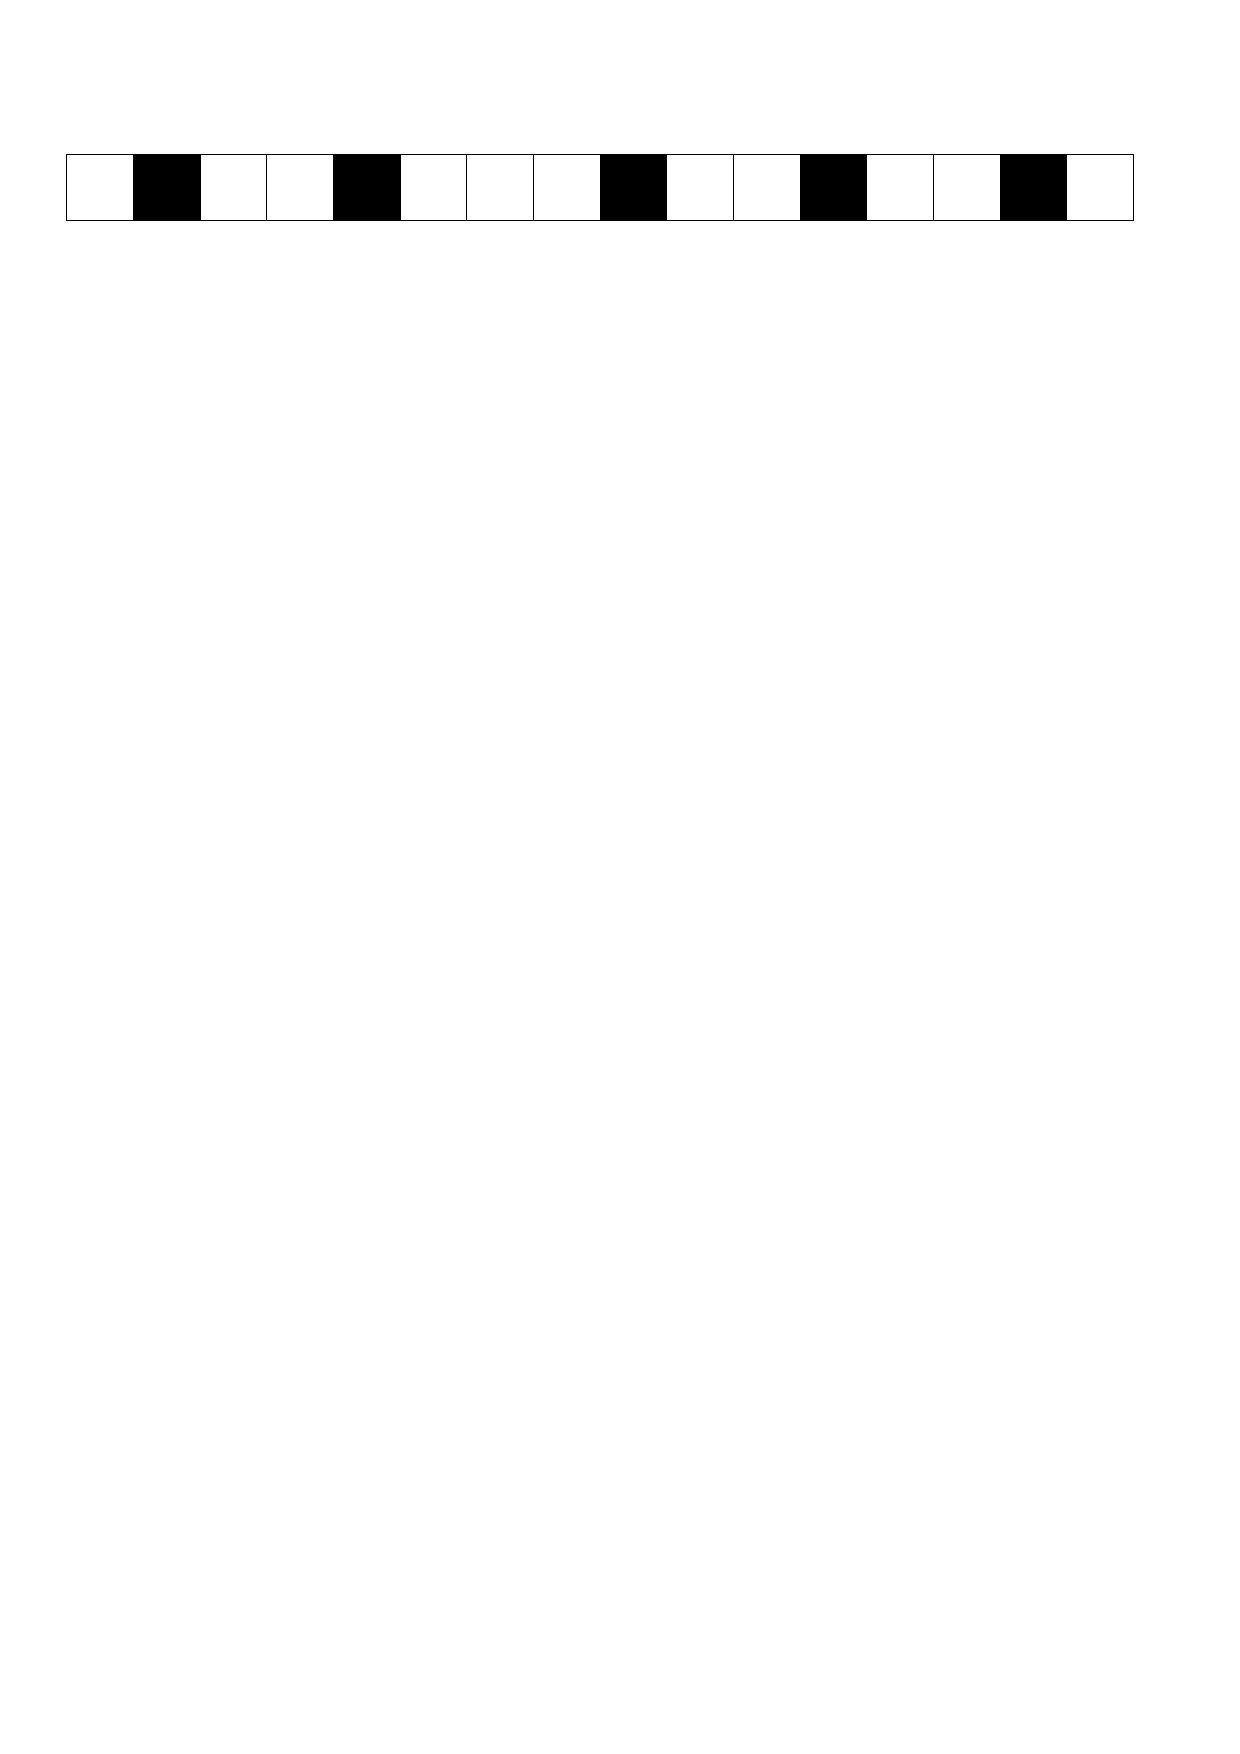
\includegraphics[width=0.9\textwidth]{./img/1Dline}
 \label{1d}
 \caption{1D cellular automaton}
\end{figure}

Range r=1 means that in update rule, 
we consider states of 3 cells. The cell itself, 
1 neighbour to the left and 1 to the right.\\

Example of an update rule is in the Table~\ref{rule90}.\\


\begin{table}[htbp]
 \centering
 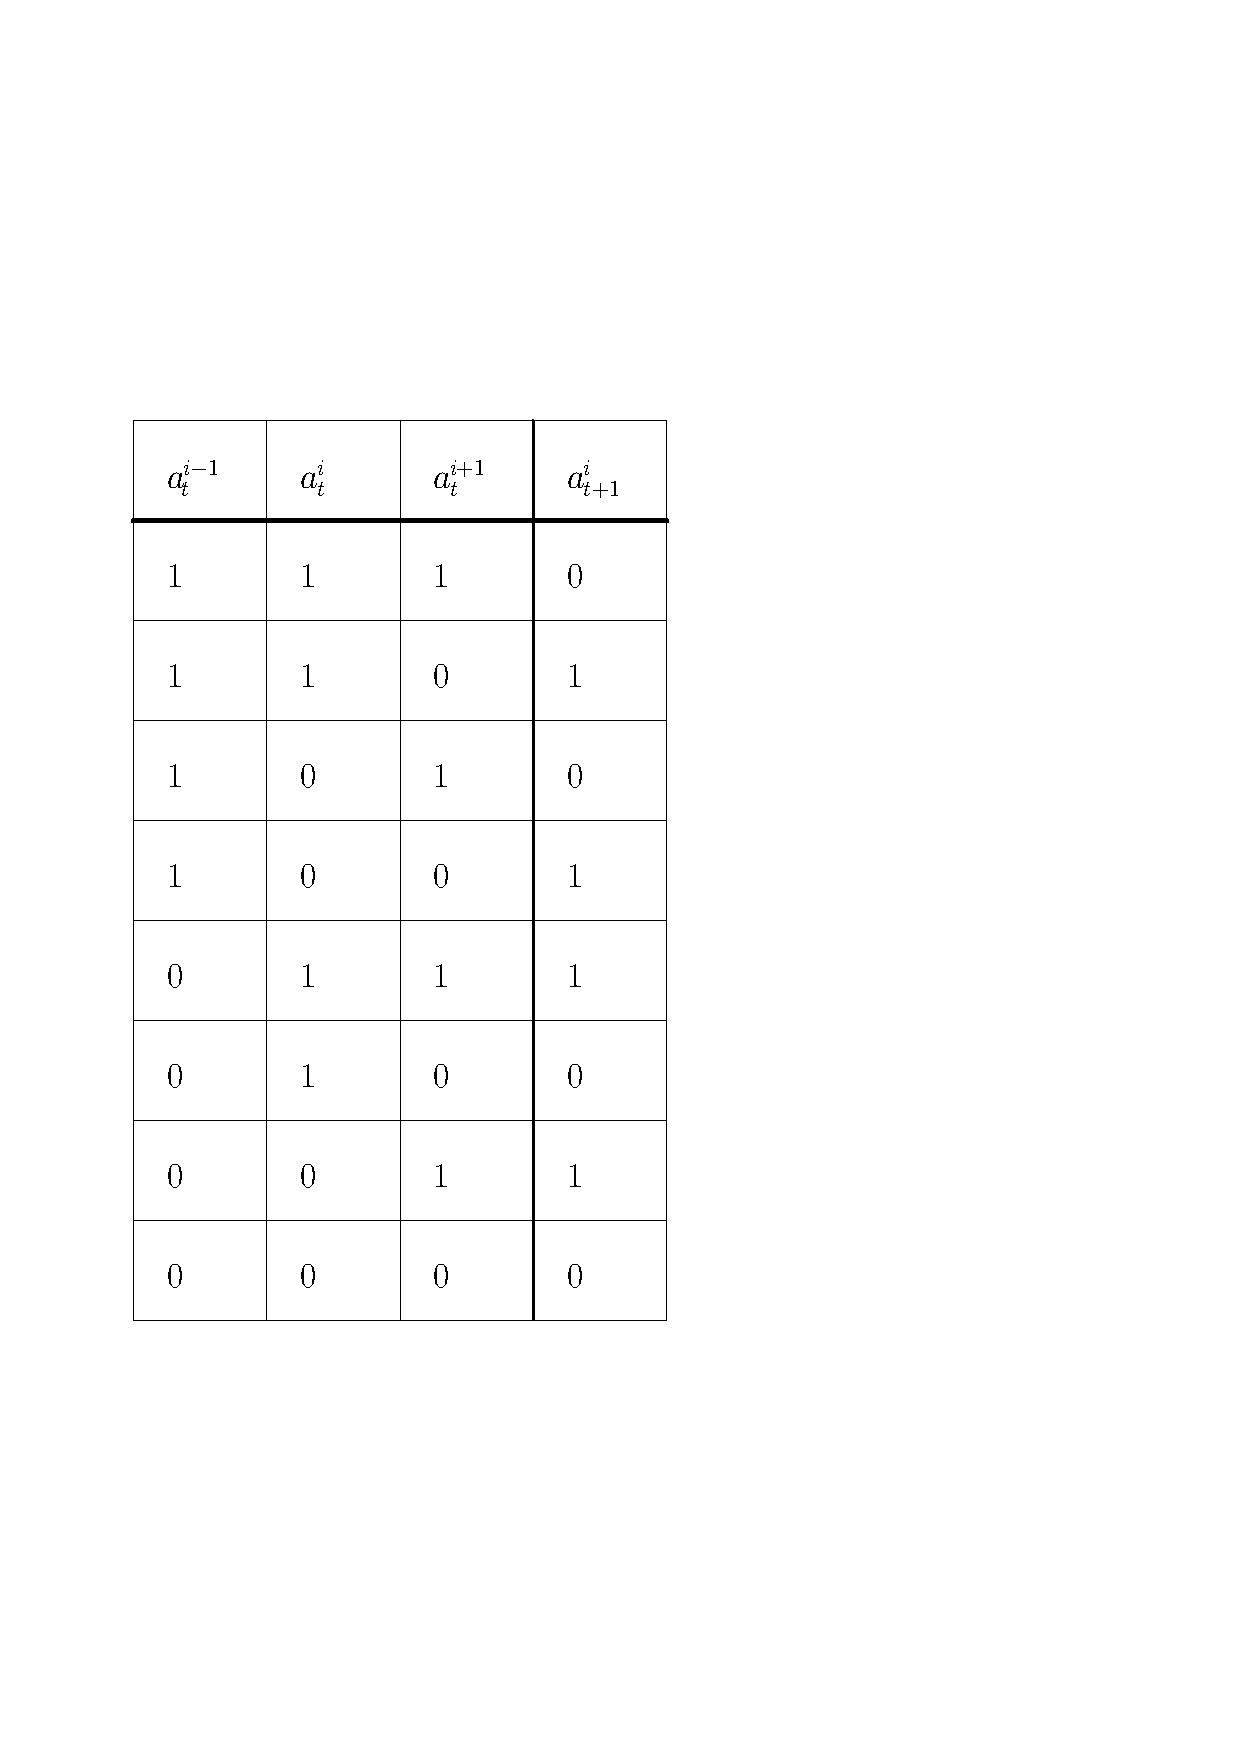
\includegraphics[width=0.4\textwidth]{./img/1Drule}
 \caption{Rule 90}
 \label{rule90}
\end{table}

%How many different update rules ("how many different Tables~\ref{rule90}")
%exist for this type of CA?

First three columns of the table denotes state of the three cells, $a_t^i$ is the middle cell and the other two are its left and right neighbor.

The rule specifies the state of the middle cell after update, based on the configuration of these three cells.
The number of possible configurations of the three cells is $2^3 = 8$.
So the rule must specify 8 bits (for each configuration one bit).
It means there are $2^8 = 256$ different rules for this most basic cellular automaton.

Let us take a look at some pictures of these cellular automata. These pictures were ploted by the simple program that we programmed for this purpose.

These pictures represent the sequences of states of cellular automata with rules 90, 30, 45 and 73.
The downer-most row is the initial configuration of CA, 
the 2nd row is configuration after 1st update etc.

\begin{figure}
 \centering
 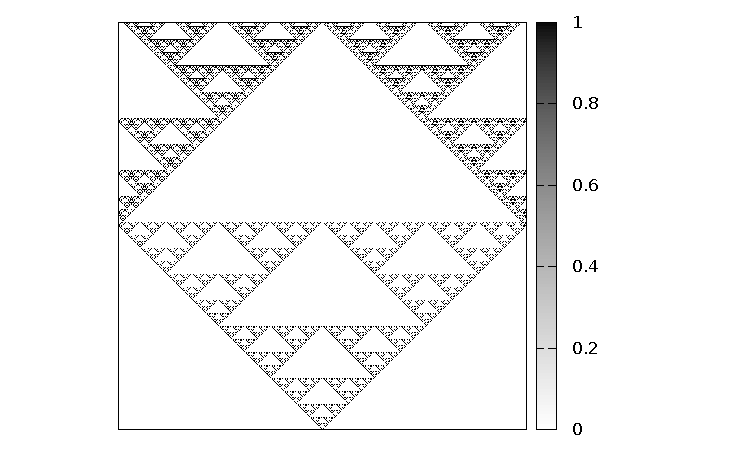
\includegraphics[width=1\textwidth]{./img/rule90}
 \caption{Rule 90}
 \label{koberec}
\end{figure}

\begin{figure}
 \centering
 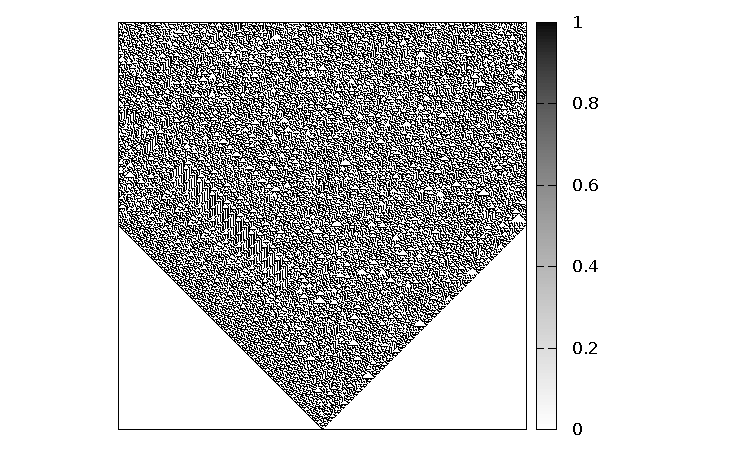
\includegraphics[width=1\textwidth]{./img/rule30}
 \caption{Rule 30}
\end{figure}

\begin{figure}
 \centering
 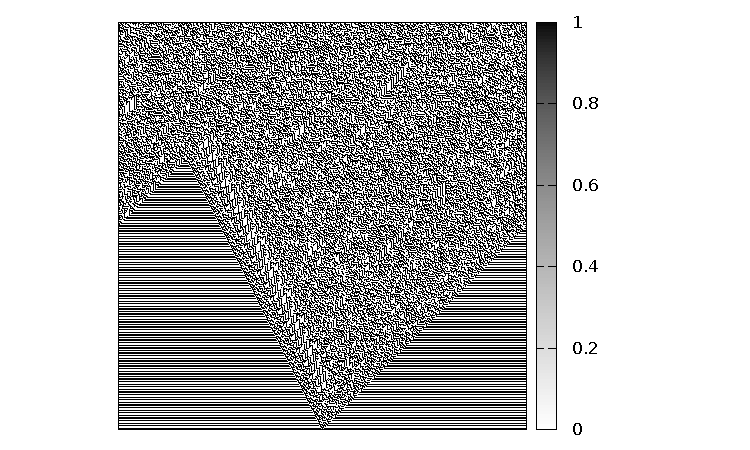
\includegraphics[width=1\textwidth]{./img/rule45}
 \caption{Rule 45}
\end{figure}

\begin{figure}
 \centering
 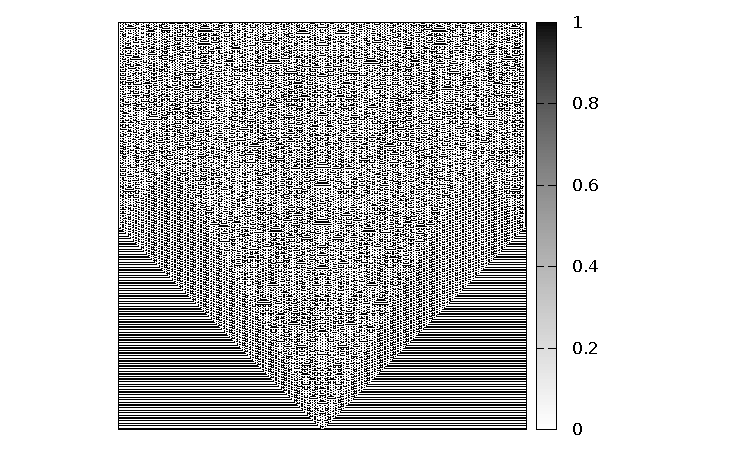
\includegraphics[width=1\textwidth]{./img/rule73}
 \caption{Rule 73}
\end{figure}

First picture~\ref{koberec} is famous fractal known as Sierpinski carpet. Wolfram classified these 1D automata into four classes, based on the regularity of the pattern obtained.

Wolfram argues that variety of behavior seen even in these most simple CA rises suspitions, and encourage hope, that in the infinitely large world of possible CAs, there is CA that model any complex phenomena you can imagine.

In his visionary book New kind of Science, Wolfram even proposes Cellular automaton that would constitute a unified theory of the fundamental physics.
Although his ideas met with rejection among theorists (see \cite{aaronson}),
many other notable physicists are attempting to construct such cellular automaton \cite{hooft}).

Some of the basic construction principles for such automata are relevant also for our models, but mostly, we would diverge too far by further exploration.
Focus of our work is much more modest that CAs describing universe.
Our focus is on CAs that model flows of the fluids.

The connection of the cellular automata with flow of fluids is not obvious or formal.
It is found on the very general level.
What connects Navier-Stokes equations and CAs are their common symettries and conservation laws implied by these symetries.
In these symmetries lies not only beauty of this method, but their strongest advantage over other well-established CFD methods.